% GNUPLOT: LaTeX picture with Postscript
\begingroup
  \makeatletter
  \providecommand\color[2][]{%
    \GenericError{(gnuplot) \space\space\space\@spaces}{%
      Package color not loaded in conjunction with
      terminal option `colourtext'%
    }{See the gnuplot documentation for explanation.%
    }{Either use 'blacktext' in gnuplot or load the package
      color.sty in LaTeX.}%
    \renewcommand\color[2][]{}%
  }%
  \providecommand\includegraphics[2][]{%
    \GenericError{(gnuplot) \space\space\space\@spaces}{%
      Package graphicx or graphics not loaded%
    }{See the gnuplot documentation for explanation.%
    }{The gnuplot epslatex terminal needs graphicx.sty or graphics.sty.}%
    \renewcommand\includegraphics[2][]{}%
  }%
  \providecommand\rotatebox[2]{#2}%
  \@ifundefined{ifGPcolor}{%
    \newif\ifGPcolor
    \GPcolorfalse
  }{}%
  \@ifundefined{ifGPblacktext}{%
    \newif\ifGPblacktext
    \GPblacktexttrue
  }{}%
  % define a \g@addto@macro without @ in the name:
  \let\gplgaddtomacro\g@addto@macro
  % define empty templates for all commands taking text:
  \gdef\gplbacktext{}%
  \gdef\gplfronttext{}%
  \makeatother
  \ifGPblacktext
    % no textcolor at all
    \def\colorrgb#1{}%
    \def\colorgray#1{}%
  \else
    % gray or color?
    \ifGPcolor
      \def\colorrgb#1{\color[rgb]{#1}}%
      \def\colorgray#1{\color[gray]{#1}}%
      \expandafter\def\csname LTw\endcsname{\color{white}}%
      \expandafter\def\csname LTb\endcsname{\color{black}}%
      \expandafter\def\csname LTa\endcsname{\color{black}}%
      \expandafter\def\csname LT0\endcsname{\color[rgb]{1,0,0}}%
      \expandafter\def\csname LT1\endcsname{\color[rgb]{0,1,0}}%
      \expandafter\def\csname LT2\endcsname{\color[rgb]{0,0,1}}%
      \expandafter\def\csname LT3\endcsname{\color[rgb]{1,0,1}}%
      \expandafter\def\csname LT4\endcsname{\color[rgb]{0,1,1}}%
      \expandafter\def\csname LT5\endcsname{\color[rgb]{1,1,0}}%
      \expandafter\def\csname LT6\endcsname{\color[rgb]{0,0,0}}%
      \expandafter\def\csname LT7\endcsname{\color[rgb]{1,0.3,0}}%
      \expandafter\def\csname LT8\endcsname{\color[rgb]{0.5,0.5,0.5}}%
    \else
      % gray
      \def\colorrgb#1{\color{black}}%
      \def\colorgray#1{\color[gray]{#1}}%
      \expandafter\def\csname LTw\endcsname{\color{white}}%
      \expandafter\def\csname LTb\endcsname{\color{black}}%
      \expandafter\def\csname LTa\endcsname{\color{black}}%
      \expandafter\def\csname LT0\endcsname{\color{black}}%
      \expandafter\def\csname LT1\endcsname{\color{black}}%
      \expandafter\def\csname LT2\endcsname{\color{black}}%
      \expandafter\def\csname LT3\endcsname{\color{black}}%
      \expandafter\def\csname LT4\endcsname{\color{black}}%
      \expandafter\def\csname LT5\endcsname{\color{black}}%
      \expandafter\def\csname LT6\endcsname{\color{black}}%
      \expandafter\def\csname LT7\endcsname{\color{black}}%
      \expandafter\def\csname LT8\endcsname{\color{black}}%
    \fi
  \fi
    \setlength{\unitlength}{0.0500bp}%
    \ifx\gptboxheight\undefined%
      \newlength{\gptboxheight}%
      \newlength{\gptboxwidth}%
      \newsavebox{\gptboxtext}%
    \fi%
    \setlength{\fboxrule}{0.5pt}%
    \setlength{\fboxsep}{1pt}%
\begin{picture}(7200.00,5040.00)%
    \gplgaddtomacro\gplbacktext{%
      \csname LTb\endcsname%
      \put(165,756){\makebox(0,0)[r]{\strut{}$0$}}%
      \csname LTb\endcsname%
      \put(165,1260){\makebox(0,0)[r]{\strut{}$0.2$}}%
      \csname LTb\endcsname%
      \put(165,1764){\makebox(0,0)[r]{\strut{}$0.4$}}%
      \csname LTb\endcsname%
      \put(165,2268){\makebox(0,0)[r]{\strut{}$0.6$}}%
      \csname LTb\endcsname%
      \put(165,2771){\makebox(0,0)[r]{\strut{}$0.8$}}%
      \csname LTb\endcsname%
      \put(165,3275){\makebox(0,0)[r]{\strut{}$1$}}%
      \csname LTb\endcsname%
      \put(165,3779){\makebox(0,0)[r]{\strut{}$1.2$}}%
      \csname LTb\endcsname%
      \put(165,4283){\makebox(0,0)[r]{\strut{}$1.4$}}%
      \csname LTb\endcsname%
      \put(360,473){\makebox(0,0){\strut{}$-1.5$}}%
      \csname LTb\endcsname%
      \put(840,473){\makebox(0,0){\strut{}$-1$}}%
      \csname LTb\endcsname%
      \put(1320,473){\makebox(0,0){\strut{}$-0.5$}}%
      \csname LTb\endcsname%
      \put(1800,473){\makebox(0,0){\strut{}$0$}}%
      \csname LTb\endcsname%
      \put(2279,473){\makebox(0,0){\strut{}$0.5$}}%
      \csname LTb\endcsname%
      \put(2759,473){\makebox(0,0){\strut{}$1$}}%
      \csname LTb\endcsname%
      \put(3239,473){\makebox(0,0){\strut{}$1.5$}}%
    }%
    \gplgaddtomacro\gplfronttext{%
      \csname LTb\endcsname%
      \put(-473,2645){\rotatebox{-270}{\makebox(0,0){\strut{}$E / \epsilon_{F,0}$}}}%
      \put(1799,143){\makebox(0,0){\strut{}$k / k_F$}}%
      \put(1799,4928){\makebox(0,0){\strut{}Imaginary interwire pairing}}%
      \csname LTb\endcsname%
      \put(1856,4307){\makebox(0,0)[l]{\strut{}$|\varepsilon_k|$}}%
      \csname LTb\endcsname%
      \put(1856,3977){\makebox(0,0)[l]{\strut{}$E_{F,k}$}}%
    }%
    \gplgaddtomacro\gplbacktext{%
      \csname LTb\endcsname%
      \put(3765,756){\makebox(0,0)[r]{\strut{} }}%
      \csname LTb\endcsname%
      \put(3765,1260){\makebox(0,0)[r]{\strut{} }}%
      \csname LTb\endcsname%
      \put(3765,1764){\makebox(0,0)[r]{\strut{} }}%
      \csname LTb\endcsname%
      \put(3765,2268){\makebox(0,0)[r]{\strut{} }}%
      \csname LTb\endcsname%
      \put(3765,2771){\makebox(0,0)[r]{\strut{} }}%
      \csname LTb\endcsname%
      \put(3765,3275){\makebox(0,0)[r]{\strut{} }}%
      \csname LTb\endcsname%
      \put(3765,3779){\makebox(0,0)[r]{\strut{} }}%
      \csname LTb\endcsname%
      \put(3765,4283){\makebox(0,0)[r]{\strut{} }}%
      \csname LTb\endcsname%
      \put(3960,473){\makebox(0,0){\strut{}$-1.5$}}%
      \csname LTb\endcsname%
      \put(4440,473){\makebox(0,0){\strut{}$-1$}}%
      \csname LTb\endcsname%
      \put(4920,473){\makebox(0,0){\strut{}$-0.5$}}%
      \csname LTb\endcsname%
      \put(5400,473){\makebox(0,0){\strut{}$0$}}%
      \csname LTb\endcsname%
      \put(5879,473){\makebox(0,0){\strut{}$0.5$}}%
      \csname LTb\endcsname%
      \put(6359,473){\makebox(0,0){\strut{}$1$}}%
      \csname LTb\endcsname%
      \put(6839,473){\makebox(0,0){\strut{}$1.5$}}%
    }%
    \gplgaddtomacro\gplfronttext{%
      \csname LTb\endcsname%
      \put(5399,143){\makebox(0,0){\strut{}$k / k_F$}}%
      \put(5399,4928){\makebox(0,0){\strut{}Real interwire pairing}}%
      \csname LTb\endcsname%
      \put(5456,4307){\makebox(0,0)[l]{\strut{}$|\varepsilon_k|$}}%
      \csname LTb\endcsname%
      \put(5456,3977){\makebox(0,0)[l]{\strut{}$E^{+}_{F,k}$}}%
      \csname LTb\endcsname%
      \put(5456,3647){\makebox(0,0)[l]{\strut{}$E^{-}_{F,k}$}}%
    }%
    \gplbacktext
    \put(0,0){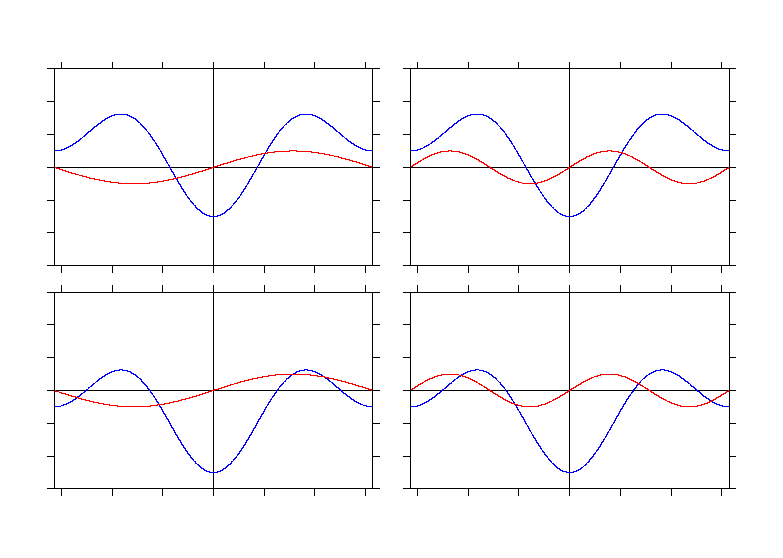
\includegraphics{Figures/twowires/Dispersionexamples/kdepend}}%
    \gplfronttext
  \end{picture}%
\endgroup
